\chapter{Benutzer-Handbuch}
\label{chap:benutzer-handbuch}

Im Benutzer-Handbuch wird die bereits fertige Anwendung beschrieben.

% \section{Ablaufbedingungen}
% \label{sec:ablaufbedingungen}

\section{Installation}
\label{sec:installation}

\textit{AntScout} benötigt keine Installation.
Das Archiv muss lediglich auf die lokale Festplatte extrahiert werden.
Dabei wird der Ordner ``AntScout'' erstellt, der alles beinhaltet, was für den Start der Anwendung nötig ist.

\section{Programm-Start}
\label{sec:programmstart}

\subsection{Voraussetzungen}
\label{sec:voraussetzungen}

\begin{itemize}
  \item Eine bestehende Internet-Verbindung.
  \item Eine möglichst aktuelle Java-Version von Oracle.
  \item Der lokale Port \texttt{8080} darf nicht durch eine bereits laufende Anwendung blockiert sein.
\end{itemize}

\subsection{Programm-Start}
\label{sec:programm-start}

\begin{enumerate}
  \item Konsole (auch Eingabeaufforderung oder Kommandozeile genannt) öffnen
  \item In das erstellte Verzeichnis ``AntScout'' wechseln
  \item \texttt{sbt}
  \item \texttt{container:start}
  \item \texttt{http://localhost:8080} oder \texttt{http://127.0.0.1:8080} im Browser aufrufen
\end{enumerate}

\subsection{Hinweise}
\label{sec:programmstart-hinweise}

\begin{itemize}
  \item Nach dem Start von \gls{sbt} werden alle benötigten Bibliotheken heruntergeladen.
    Je nach Internet-Verbindung kann dieser Vorgang mehrere Minuten dauern.
  \item Nach der Eingabe von \texttt{container:start} werden die benötigten Karten heruntergeladen und vorverarbeitet.
    Dieser Vorgang kann auch je nach Internet-Verbindung und Computer-Leistung mehrere Minuten dauern.
  \item Es sollte nach Möglichkeit ein möglichst moderner Browser, der HTML5 unterstützt, verwendet werden.
\end{itemize}

\section{Programm-Ende}
\label{sec:programm-ende}

\begin{enumerate}
  \item \texttt{container:stop}
  \item \texttt{exit}
\end{enumerate}

oder einfach die Konsole schliessen.

\section{Bedienungsanleitung}
\label{sec:bedienungsanleitung}

\subsection{Front-End}
\label{sec:front-end}

Nach dem Aufruf \texttt{http://localhost:8080} im Browser öffnet sich die Start-Seite.
Ein Screenshot dieser Seite ist in der Abbildung \ref{fig:start-seite} zu sehen.

\begin{figure}[htbp]
  \centering
  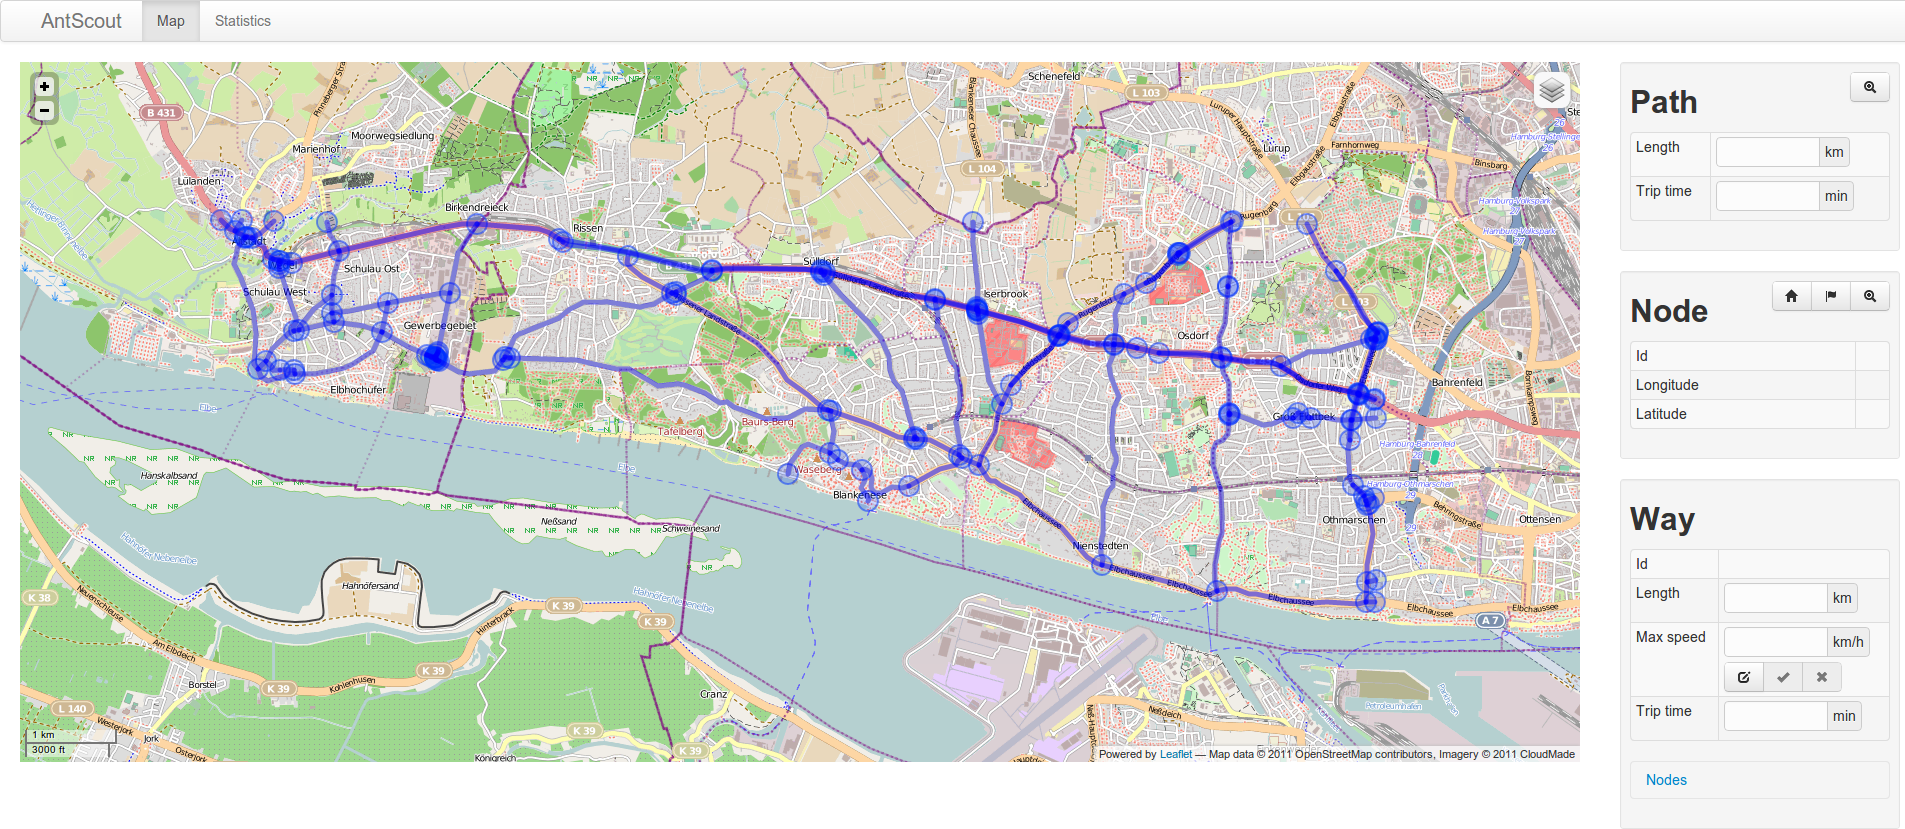
\includegraphics[width=\textwidth]{Bilder/Start-Seite.png}
  \caption{Start-Seite}
  \label{fig:start-seite}
\end{figure}

Die Seite ist in drei Bereiche unterteilt:

\begin{itemize}
  \item Menü
  \item Karte
  \item Informationen
\end{itemize}

\subsubsection{Menü}
\label{sec:menue}

Die obere Leiste stellt das Menü dar.
Hier kann zwischen der Karten- und der Statistiken-Ansicht (siehe Abschnitt \ref{sec:statistiken}) umgeschaltet werden.

\subsubsection{Karte}
\label{sec:karte}

Die Karte nimmt den größten Platz der Seite ein.
Hier sind die Kreuzungen - nachfolgend Knoten genannt - zu sehen, zwischen denen navigiert werden kann und die Wege, die die Knoten verbinden.
Jeder Knoten und jeder Weg kann durch einen Maus-Klick markiert werden.
Dieser wird dann optisch hervorgehoben.

\subsubsection{Informationen}
\label{sec:informationen}

Der Informationen-Bereich auf der rechten Seite ist in drei weitere Bereiche unterteilt:

\begin{itemize}
  \item Pfad-Informationen
  \item Knoten-Informationen
  \item Weg-Informationen
\end{itemize}

\paragraph{Pfad-Informationen}
\label{sec:pfad-informationen}

Wenn ein Pfad gefunden wurde, werden hier die Länge und die Passier-Zeit angezeigt (siehe Abbildung \ref{fig:pfad-informationen}).
Mit dem Button rechts oben können weitere Informationen eingeblendet werden.

\begin{figure}[htbp]
  \centering
  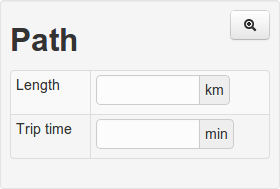
\includegraphics[width=0.4\textwidth]{Bilder/Pfad-Informationen.png}
  \caption{Pfad-Informationen}
  \label{fig:pfad-informationen}
\end{figure}

\paragraph{Knoten-Informationen}
\label{sec:knoten-informationen}

Nach der Markierung eines Knotens werden in diesem Bereich die Knoten-Daten eingetragen.
Es handelt sich um die Id und die geographischen Daten, die direkt aus \gls{osm} übernommen werden (siehe Abbildung \ref{fig:knoten-informationen}).

\begin{figure}[htbp]
  \centering
  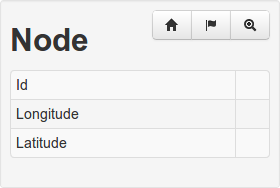
\includegraphics[width=0.4\textwidth]{Bilder/Knoten-Informationen.png}
  \caption{Knoten-Informationen}
  \label{fig:knoten-informationen}
\end{figure}

Die drei Buttons rechts oben im Knoten-Informationen-Bereich (siehe Abbildung \ref{fig:knoten-buttons}) führen verschiedene Aktionen aus.
Mit dem linken kann der aktuell selektierte Knoten als Start und mit dem mittleren als Ziel gesetzt werden.
Ein als Start oder Ziel gesetzter Knoten wird mit einem entsprechenden Marker versehen (siehe Abbildungen \ref{fig:start-knoten} und \ref{fig:ziel-knoten}).
Mit dem rechten Button können weitere Informationen über die aktuell selektierte Knoten-Konstellation eingeblendet werden.

\begin{figure}[htbp]
  \centering
  
\includegraphics[width=0.15\textwidth]{Bilder/Knoten-Buttons.png}
  \caption{Knoten-Buttons}
  \label{fig:knoten-buttons}
\end{figure}

\begin{figure}[htbp]
  \centering
  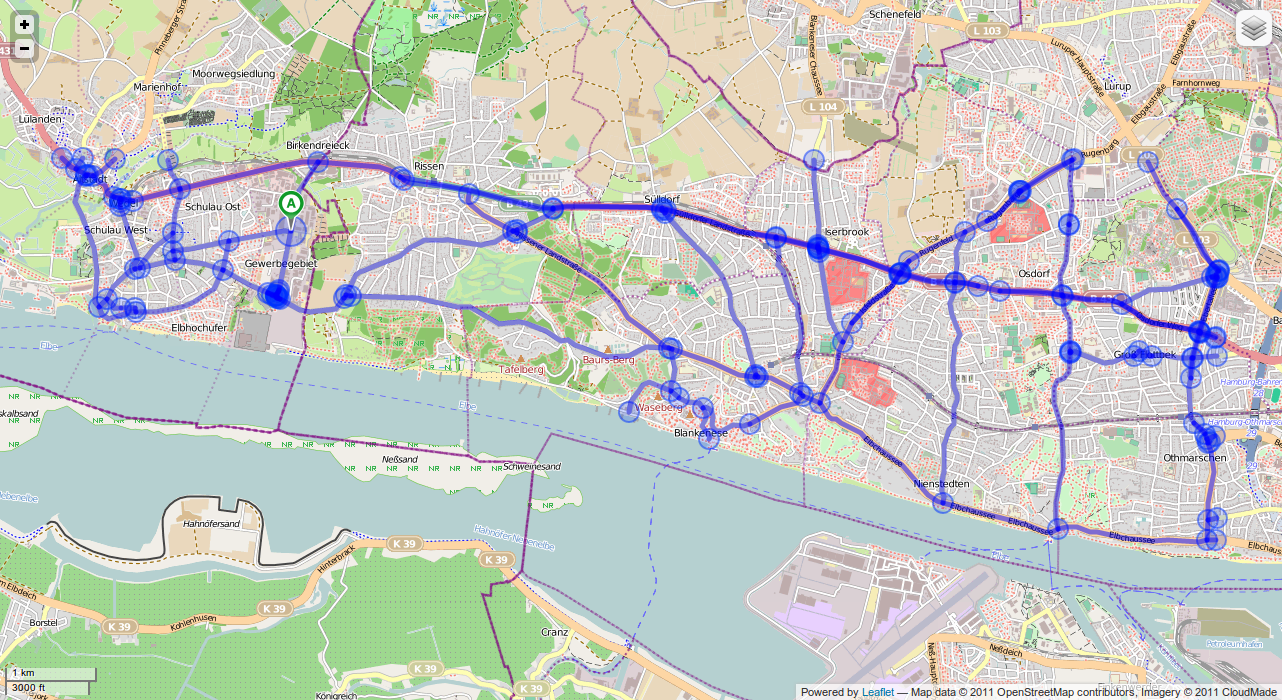
\includegraphics[width=\textwidth]{Bilder/Start-Knoten.png}
  \caption{Start-Knoten}
  \label{fig:start-knoten}
\end{figure}

\begin{figure}[htbp]
  \centering
  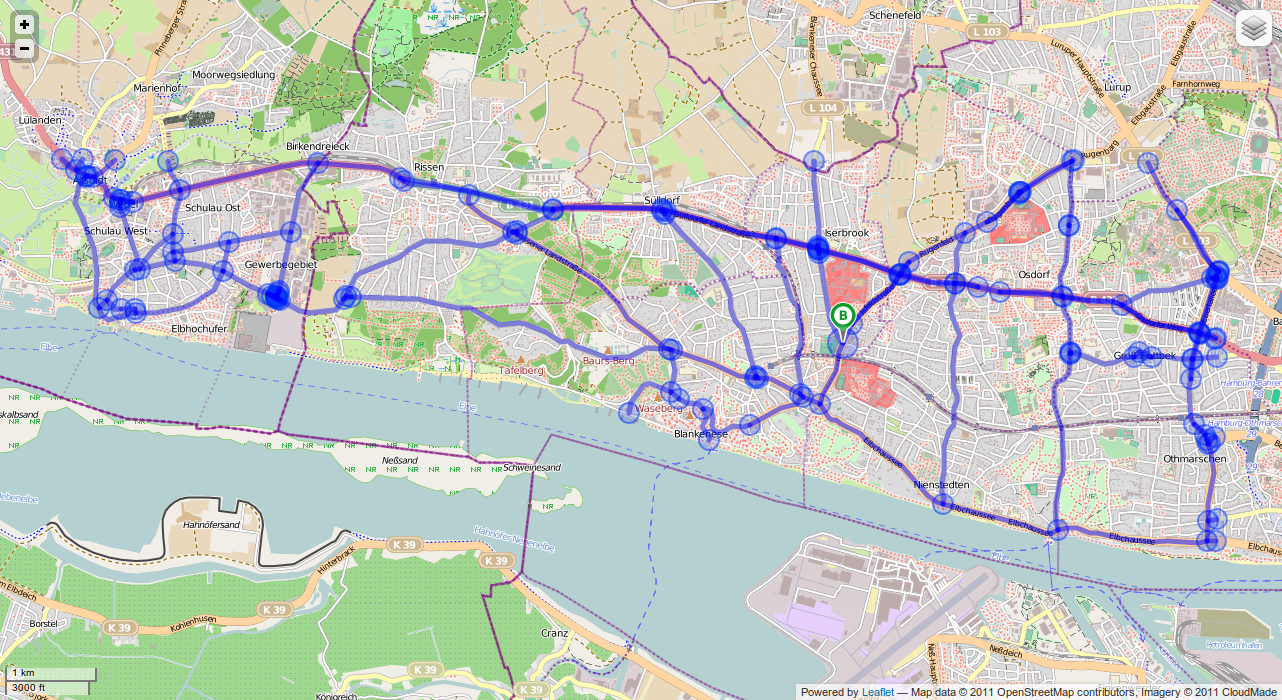
\includegraphics[width=\textwidth]{Bilder/Ziel-Knoten.png}
  \caption{Ziel-Knoten}
  \label{fig:ziel-knoten}
\end{figure}

\paragraph{Weg-Informationen}
\label{sec:weg-informationen}

Hier werden die Daten eines selektierten Weges angezeigt.
Neben einer Weg-Id werden hier die Länge, die aktuell maximale Geschwindigkeit des Weges, die Passier-Zeit und die Knoten angezeigt, aus denen der Weg besteht (siehe Abbildung \ref{fig:weg-informationen}).
Die Knoten können durch einen Klick auf ``Nodes'' eingeblendet werden.

Unter der maximalen Geschwindigkeit sind drei Buttons zu sehen (siehe Abbildung \ref{fig:weg-editier-buttons}).
Mit diesen Buttons kann die maximale Geschwindigkeit editiert werden.
Der linke Button schaltet in den Editier-Modus.
Im Editier-Modus ist die maximale Geschwindigkeit editierbar und die beiden rechten Buttons sind aktiv.
Anschließend kann die neue Geschwindigkeit eingegeben werden.
Mit dem mittleren Button kann diese gespeichert werden.
Mit dem rechten Button wird der Editier-Modus verlassen, ohne die Änderung zu übernehmen.

\begin{figure}[htbp]
  \centering
  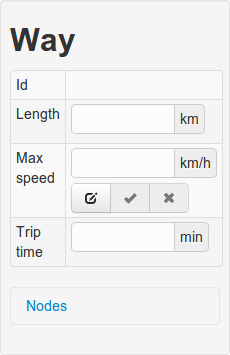
\includegraphics[width=0.3\textwidth]{Bilder/Weg-Informationen.png}
  \caption{Weg-Informationen}
  \label{fig:weg-informationen}
\end{figure}

\begin{figure}[htbp]
  \centering
  
\includegraphics[width=0.15\textwidth]{Bilder/Weg-Editier-Buttons.png}
  \caption{Weg-Editier-Buttons}
  \label{fig:weg-editier-buttons}
\end{figure}

\subsubsection{Statistiken}
\label{sec:statistiken}

In der Statistiken-Ansicht kann der aktuelle Zustand des Systems abgelesen werden.
Diese ist in drei Bereiche unterteilt (Abbildung \ref{fig:statistiken}):

\begin{itemize}
  \item Ameisen-Statistiken (Abbildung \ref{fig:ameisen-statistiken})
  \item Knoten-Statistiken (Abbildung \ref{fig:knoten-statistiken})
  \item Zeit-Punkt der letzten Aktualisierung (Abbildung \ref{fig:letztes-update})
\end{itemize}

\begin{figure}[htbp]
  \centering
  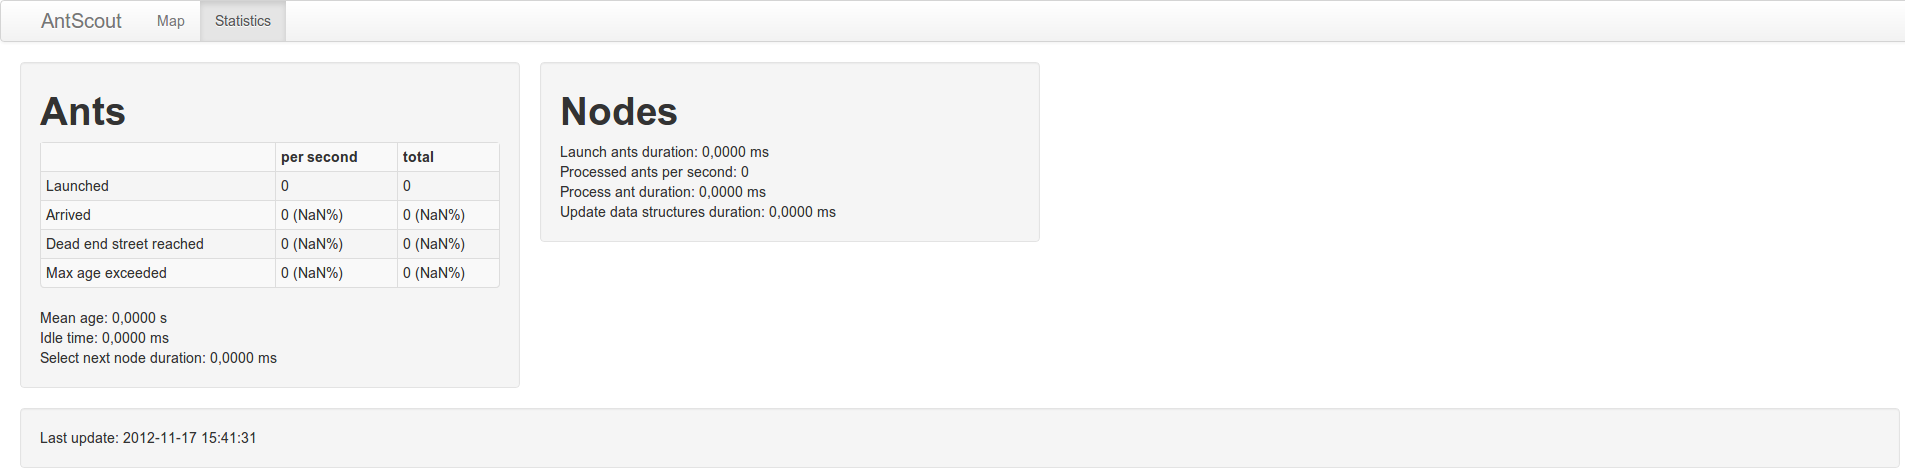
\includegraphics[width=\textwidth]{Bilder/Statistiken.png}
  \caption{Statistiken}
  \label{fig:statistiken}
\end{figure}

\subsubsection{Ameisen-Statistiken}
\label{sec:ameisen-statistiken}

In diesem Bereich ist oben eine Tabelle zu sehen.
In dieser ist jeweils die Anzahl der erzeugten, der das Ziel erreichten, der in einer Sack-Gasse angekommenen und der das maximale Alter überschrittenen Ameisen aufgeführt.
Es wird sowohl die Anzahl pro Sekunde als auch die Gesamt-Anzahl angezeigt.
Unter der Tabelle ist das durchschnittliche Ameisen-Alter, die Leerlauf-Zeit der Ameisen und die Zeit, die zum Auswählen des nächsten Knotens benötigt wurde, angezeigt.

\begin{figure}[htbp]
  \centering
  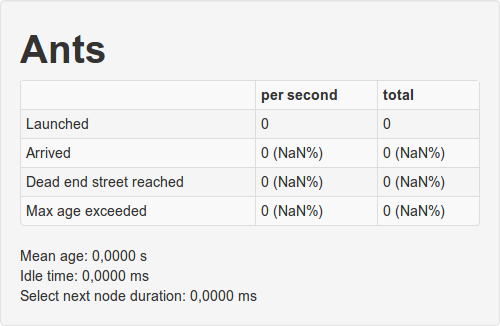
\includegraphics[width=0.7\textwidth]{Bilder/Ameisen-Statistiken.png}
  \caption{Ameisen-Statistiken}
  \label{fig:ameisen-statistiken}
\end{figure}

\subsubsection{Knoten-Statistiken}
\label{sec:Knoten-statistiken}

Hier sind folgende Angaben zu finden:

\begin{itemize}
  \item Durchschnittliche Dauer, die zum Erzeugen von Ameisen benötigt wird.
  \item Durchschnittliche Anzahl der Ameisen, die ein Knoten pro Sekunde verarbeitet.
  \item Durchschnittliche Dauer, die für die Verarbeitung einer Ameise nötig ist.
  \item Durchschnittliche Dauer, die für die Aktualisierung der Knoten-Daten-Strukturen gebraucht wird.
\end{itemize}

\begin{figure}[htbp]
  \centering
  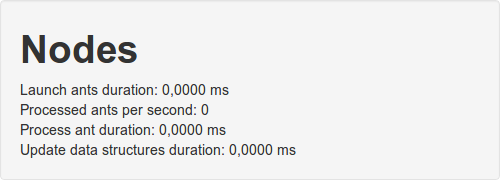
\includegraphics[width=0.7\textwidth]{Bilder/Knoten-Statistiken.png}
  \caption{Knoten-Statistiken}
  \label{fig:knoten-statistiken}
\end{figure}

\begin{figure}[htbp]
  \centering
  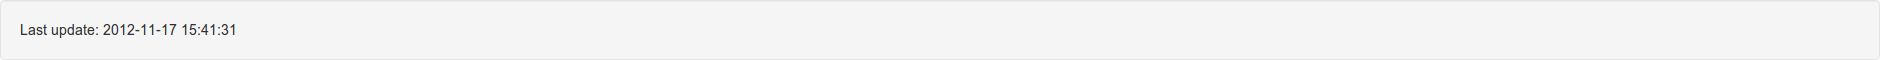
\includegraphics[width=\textwidth]{Bilder/Letztes-Update.png}
  \caption{Letztes Update}
  \label{fig:letztes-update}
\end{figure}

\subsection{Routing}
\label{sec:routing}

Wenn sowohl Start als auch Ziel wie in Abschnitt \ref{sec:knoten-informationen} beschrieben gesetzt wurden, sucht \textit{AntScout} eine Route vom Start zum Ziel und zeigt diese an (Abbildung \ref{fig:route}).
Jetzt kann einer der Wege, der auf der Route liegt selektiert und dessen maximale Geschwindigkeit wie in Abschnitt \ref{sec:weg-informationen} beschrieben verändert werden.
Eine starke Verringerung der Geschwindigkeit veranlasst das System nach einer schnelleren Route zu suchen und diese anzuzeigen (Abbildung \ref{fig:alternative-route}).

\begin{figure}[htbp]
  \centering
  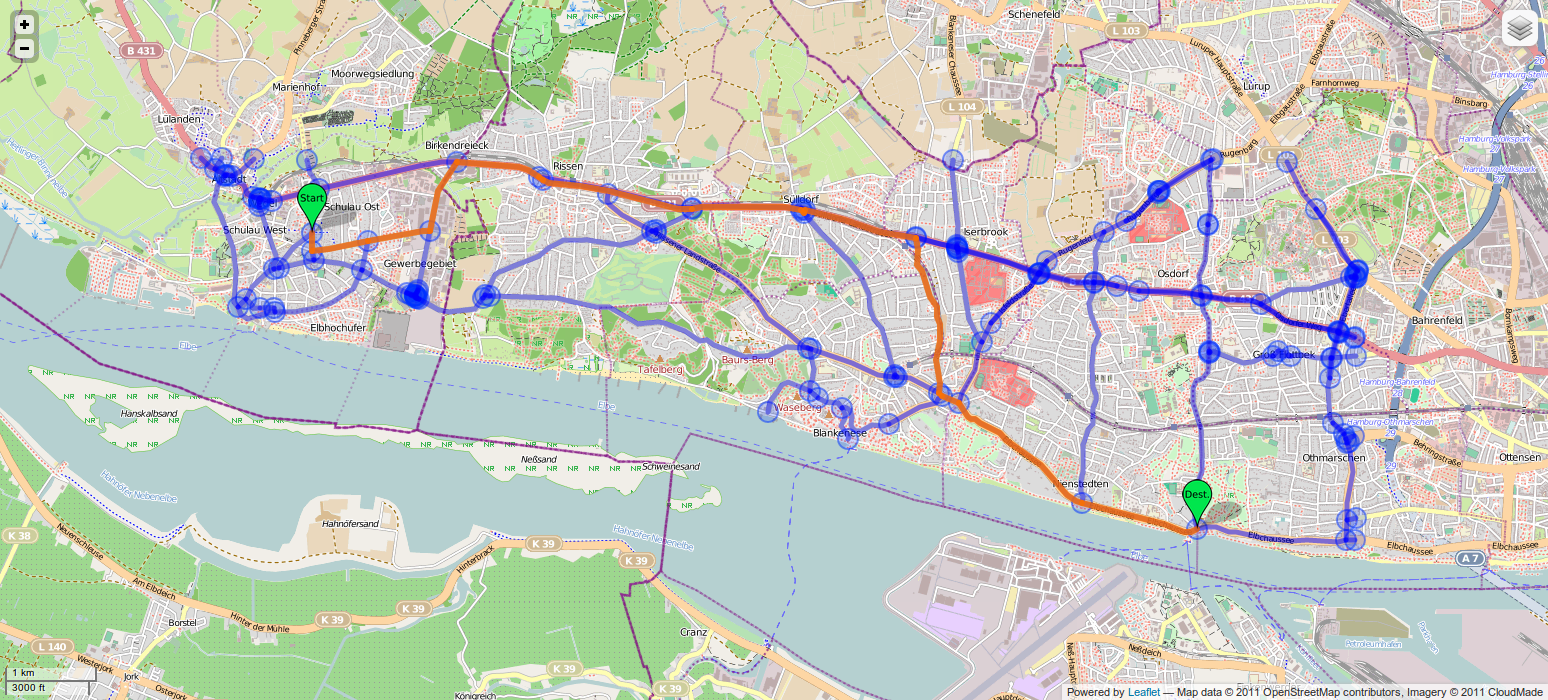
\includegraphics[width=\textwidth]{Bilder/Route.png}
  \caption{Route}
  \label{fig:route}
\end{figure}

\begin{figure}[htbp]
  \centering
  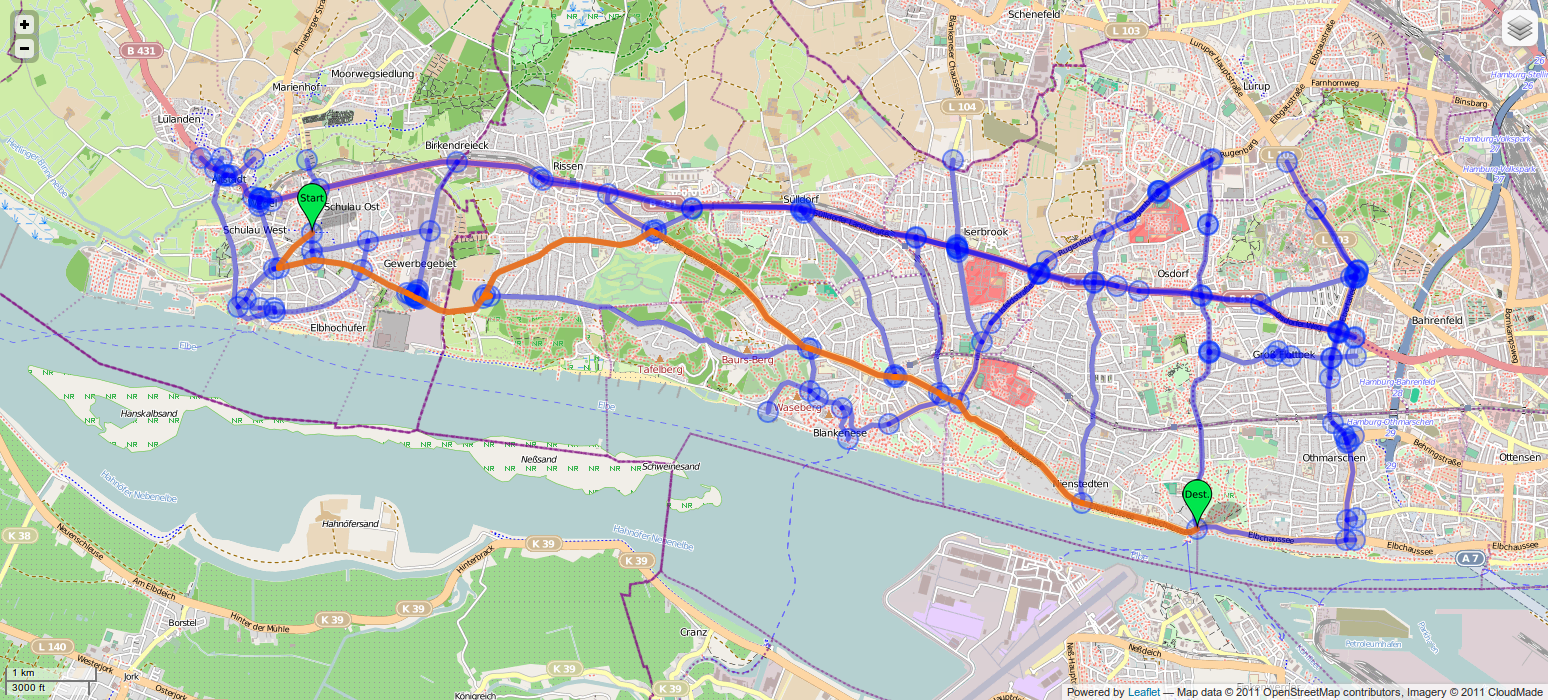
\includegraphics[width=\textwidth]{Bilder/Alternative-Route.png}
  \caption{Alternative-Route}
  \label{fig:alternative-route}
\end{figure}

\subsection{Konfiguration}
\label{sec:konfiguration}

\textbf{Achtung!}
Hier sollten nur fortgeschrittene Benutzer etwas ändern.
Es besteht die Gefahr einer ungültigen Konfiguration.
Dann gibt \textit{AntScout} beim Starten eine Fehlermeldung aus und startet nicht mehr richtig.

Im Verzeichnis \texttt{AntScout/src/main/resources} befindet sich die Datei \texttt{reference.conf}.
Dort sind die Einstellungen für \textit{AntScout} zu finden.
Die Datei ist eine Text-Datei und kann mit einem Text-Editor bearbeitet werden.

Die Konfiguration ist in mehrere Ebenen unterteilt, wobei \texttt{ant-scout} die oberste Ebene darstellt.
Jede ebene ist in geschweifte Klammern eingeschlossen.

Jeder Parameter ist durch einen Namen und einen Wert definiert.

\begin{lstlisting}
name = wert
\end{lstlisting}

Jede Änderung der Konfiguration wird erst nach einem Neustart der Applikation wirksam.

\begin{description}
  \item[ant-net] In diesem Abschnitt können die Parameter angepasst werden, die die Arbeitsweise von \textit{AntNet} - des im Hintergrund arbeitenden Routing-Algorithmus - beeinflussen.
    Diese Parameter werden in den nächsten Abschnitten nur grob beschrieben.
    Detailliertere Ausführungen sind in der entsprechenden Literatur (\cite{DorigoStuetzle2004} oder \cite{Walther2006}) zu finden.
    \begin{description}
      \item[a] Parameter \texttt{a} für die Squash-Funktion.
      \item[alpha] Relatives Gewicht der heuristischen Information, die in die Berechnung der Wahrscheinlichkeiten einfließt.
      \item[ants-launch] Parameter, die zum Erzeugen der Ameisen benötigt werden.
        \begin{description}
          \item[group-distance] Die von einem Knoten aus erreichbaren Ziele werden in Gruppen unterteilt.
            Dieser Parameter (Angabe in Metern) entscheidet, in welchen Abständen eine neue Gruppe erzeugt wird.
          \item[initial-delay] Intervall in Millisekunden, in dem Ameisen mit Zielen aus der am weitesten entfernten Gruppe erzeugt werden.
          \item[delay-increment] Mit abnehmender Entfernung wird pro Gruppe dieser Wert (Angabe in Millisekunden) zum \texttt{initial-delay} hinzu addiert.
        \end{description}
      \item[max-ant-age] Maximales Alter einer Ameise in Millisekunden.
        Wenn die Ameise ihr Ziel nicht innerhalb dieser Zeit erreicht hat, wird sie aus dem System entfernt.
      \item[best-way-pheromone] Mit diesem Wert wird der beste Weg in der Pheromon-Matrix initialisiert, der als nächstes auf dem Weg zum Ziel besucht werden sollte.
      \item[c1] Gewichtungsfaktor, der den Einfluss des Verhältnisses der besten Fahrzeit zur aktuellen Fahrzeit bei der Berechnung der Verstärkung angibt.
      \item[c2] Gewichtungsfaktor, der den Einfluss der Vertrauenswürdigkeit der aktuellen Fahrzeit bei der Berechnung der Verstärkung angibt.
      \item[varsigma] Faktor, der die Anzahl der Messungen bestimmt, die zum Berechnen des Mittelwertes und der Varianz des lokalen statistischen Modells verwendet werden.
      \item[w-max] Größe des gleitendes Beobachtungsfensters des lokalen statistischen Modells.
        Sollte nach \cite{DorigoStuetzle2004} wie folgt berechnet werden: $w-max = 5 \frac{c}{varsigma}$ mit $c <= 1$.
      \item[z] Parameter \texttt{z} für die Berechnung der Verstärkung.
    \end{description}
  \item[default-speeds] Standard-Geschwindigkeiten für verschiedene \gls{osm}-Weg-Klassen.
    Diese Geschwindigkeiten werden den Wegen zugewiesen, wenn in der \gls{osm}-Weg-Definition keine maximale Geschwindigkeit definiert ist.
  \item[epsilon] Schwellwert für den Vergleich von zwei Double-Werten.
  \item[map] Dieser Parameter steuert, welche Karte verwendet werden soll.
    Es sind mehrere Karten in verschiedenen Größen vordefiniert.
    Die Zeile, die die aktuell verwendete Karte enthält, ist die einzige, die nicht mit einem \#-Zeichen beginnt.
    Dieser Zeile muss ein \#-Zeichen vorangestellt werden, damit sie nicht mehr verwendet wird.
    Vor der Zeile, die die gewünschte Karte enthält, muss das \#-Zeichen entfernt werden.
    \begin{lstlisting}
# Karte, die verwendet werden soll.
# 104 Knoten, 99 Quellen und 100 Ziele
# map = maps/Bahrenfeld-Gross-Flottbek-Othmarschen-Ottensen.osm
# 85 Knoten, 83 Quellen und 83 Ziele
# map = maps/Blankenese-Wedel.osm
# 47 Knoten, 43 Quellen und 45 Ziele
map = maps/Altona-50-Knoten.osm
# 14 Knoten, 12 Quellen und Ziele
# map = maps/Altona-Kreis.osm
# 142 Knoten, 138 Quellen und Ziele
# map = maps/Altona-Wedel.osm
# 57 Knoten, 57 Quellen und 56 Ziele
# map = maps/Wedel.osm
    \end{lstlisting}
  \item[max-path-length] Die Suche nach einem Pfad wird abgebrochen, wenn der Pfad diese Länge erreicht.
  \item[process-statistics-delay] Intervall in Sekunden, in dem Statistiken erzeugt und verarbeitet werden.
    Der Wert 0 schaltet die Statistiken aus.
    Statistiken senken die Performance und sollten nur wenn nötig eingeschaltet werden!
  \item[relevant-highways] \gls{osm}-Weg-Klassen, die für den AntNet-Algorithmus berücksichtigt werden sollen.
  \item[trace-is-enabled] Flag, ob detaillierte (Log-)Ausgaben erzeugt werden sollen.
    Senkt die Performance und sollte nur zur Fehlersuche eingeschaltet werden!
\end{description}

% \section{Fehlermeldungen}
% \label{sec:fehlermeldungen}

\section{Wiederanlaufbedingungen}
\label{sec:wiederanlaufbedingungen}

Sollte die Anwendung einmal abstürzen oder/und nicht mehr reagieren, kann sie wie in Abschnitt \ref{sec:programm-ende} beschrieben beendet werden.
In Abschnitt \ref{sec:programm-ende} ist geschildert, wie die Anwendung erneut gestartet werden kann.
